\item O avião a jato de \SI{12}{\mega\g} é capaz de decolar verticalmente sobre o tombadilho de um avião. Se o seu jato exerce uma força vertical constante de \SI{150}{\kilo\newton} sobre o plano, determine sua velocidade e a altura a que chegará em $t=\SI{6}{\second}$, partindo do repouso. Despreze a perda de combustível durante a subida.

\import{sections/answers/}{answer-1}

\vspace{-1.7cm}
\begin{flushright}
	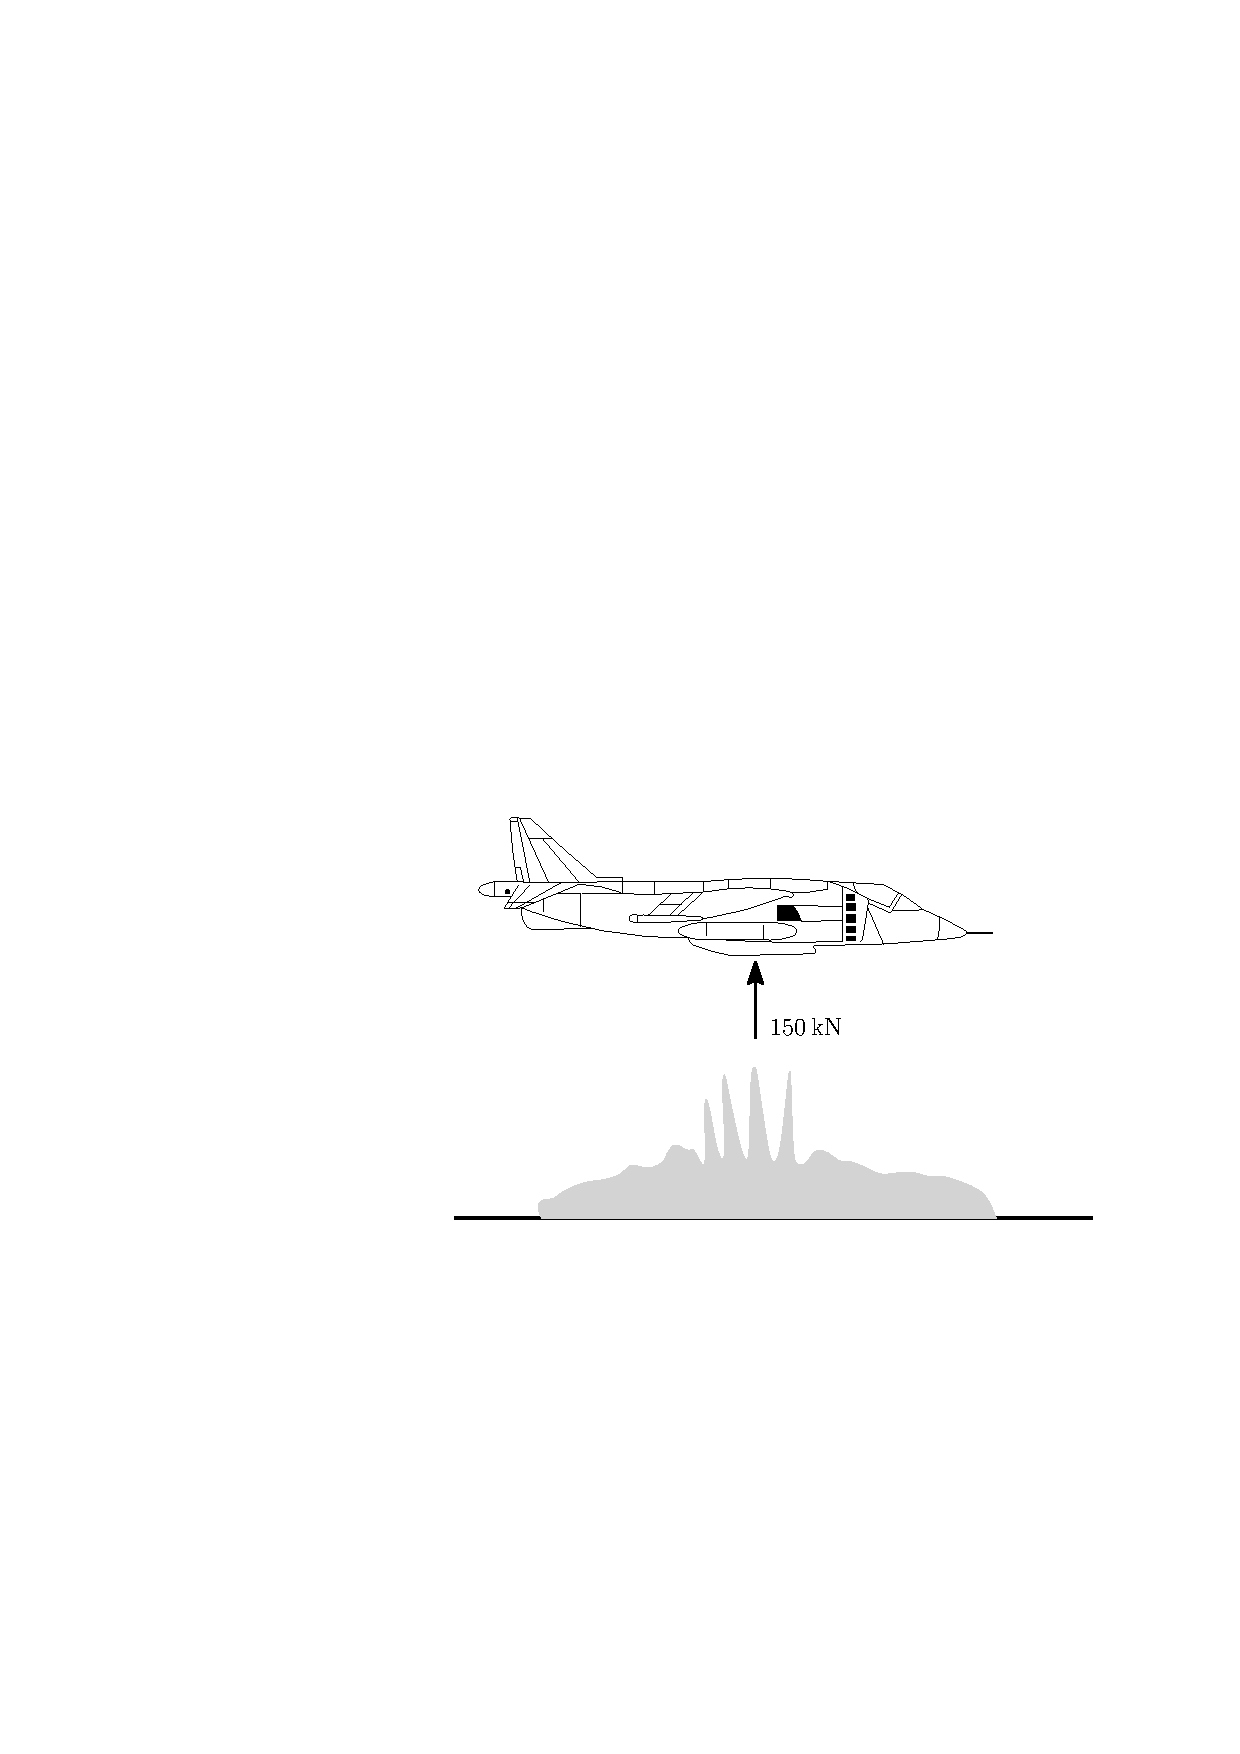
\includegraphics[scale=.8]{images/draw_1}
\end{flushright}